\documentclass[]{article}
\usepackage{lmodern}
\usepackage{amssymb,amsmath}
\usepackage{ifxetex,ifluatex}
\usepackage{fixltx2e} % provides \textsubscript
\ifnum 0\ifxetex 1\fi\ifluatex 1\fi=0 % if pdftex
  \usepackage[T1]{fontenc}
  \usepackage[utf8]{inputenc}
\else % if luatex or xelatex
  \ifxetex
    \usepackage{mathspec}
  \else
    \usepackage{fontspec}
  \fi
  \defaultfontfeatures{Ligatures=TeX,Scale=MatchLowercase}
\fi
% use upquote if available, for straight quotes in verbatim environments
\IfFileExists{upquote.sty}{\usepackage{upquote}}{}
% use microtype if available
\IfFileExists{microtype.sty}{%
\usepackage{microtype}
\UseMicrotypeSet[protrusion]{basicmath} % disable protrusion for tt fonts
}{}
\usepackage[margin=1in]{geometry}
\usepackage{hyperref}
\hypersetup{unicode=true,
            pdftitle={Predicting Household Composition by TV Viewing Behavior},
            pdfauthor={Rafael Lüchinger},
            pdfborder={0 0 0},
            breaklinks=true}
\urlstyle{same}  % don't use monospace font for urls
\usepackage{graphicx,grffile}
\makeatletter
\def\maxwidth{\ifdim\Gin@nat@width>\linewidth\linewidth\else\Gin@nat@width\fi}
\def\maxheight{\ifdim\Gin@nat@height>\textheight\textheight\else\Gin@nat@height\fi}
\makeatother
% Scale images if necessary, so that they will not overflow the page
% margins by default, and it is still possible to overwrite the defaults
% using explicit options in \includegraphics[width, height, ...]{}
\setkeys{Gin}{width=\maxwidth,height=\maxheight,keepaspectratio}
\IfFileExists{parskip.sty}{%
\usepackage{parskip}
}{% else
\setlength{\parindent}{0pt}
\setlength{\parskip}{6pt plus 2pt minus 1pt}
}
\setlength{\emergencystretch}{3em}  % prevent overfull lines
\providecommand{\tightlist}{%
  \setlength{\itemsep}{0pt}\setlength{\parskip}{0pt}}
\setcounter{secnumdepth}{5}
% Redefines (sub)paragraphs to behave more like sections
\ifx\paragraph\undefined\else
\let\oldparagraph\paragraph
\renewcommand{\paragraph}[1]{\oldparagraph{#1}\mbox{}}
\fi
\ifx\subparagraph\undefined\else
\let\oldsubparagraph\subparagraph
\renewcommand{\subparagraph}[1]{\oldsubparagraph{#1}\mbox{}}
\fi

%%% Use protect on footnotes to avoid problems with footnotes in titles
\let\rmarkdownfootnote\footnote%
\def\footnote{\protect\rmarkdownfootnote}

%%% Change title format to be more compact
\usepackage{titling}

% Create subtitle command for use in maketitle
\providecommand{\subtitle}[1]{
  \posttitle{
    \begin{center}\large#1\end{center}
    }
}

\setlength{\droptitle}{-2em}

  \title{Predicting Household Composition by TV Viewing Behavior}
    \pretitle{\vspace{\droptitle}\centering\huge}
  \posttitle{\par}
  \subtitle{Diploma of Advanced Studies in Applied Statistics at ETH Zurich}
  \author{Rafael Lüchinger}
    \preauthor{\centering\large\emph}
  \postauthor{\par}
      \predate{\centering\large\emph}
  \postdate{\par}
    \date{09 April 2019}

\usepackage{float}

\begin{document}
\maketitle

{
\setcounter{tocdepth}{2}
\tableofcontents
}
\section{Abstract}\label{abstract}

\section{Introduction}\label{introduction}

TV audiance in Switzerland is measured by
\href{https:://www.mediapulse.ch/en}{Mediapulse AG}. A representative
\href{https:://www.mediapulse.ch/en/tv/research-method/the-panel.html}{panel}
of roughly 2000 households is constantly under
\href{https:://www.mediapulse.ch/en/tv/research-method/the-measuring-technique.html}{measurement}.
These homes were carfully selected by a complex sampling design and all
householdmembers have agreed to be part of the study. The TV viewing of
each householdmember is individually recorded and detailed demografics
are known for each person. This allows the market to target TV audiances
by relevant characteristics like age gender and many more.

One issue with the panel approach is poor granularity. That means
sometimes the system can not provide any audiance figures for a specific
channel or airtime. It is likely that in the Swiss population of about
3.5 Mio. households at least a few people are watching even exotic
programs at exotic times of the day. However, out of a panel of 2000
households chances are high that no one was watching that content. This
is not a bias of the measurement but poor resolution.

A solution to this problem could be the inclusion of third party data.
Set-Top-Boxes (STB) of TV-provider (Swisscom, UPC, etc.) are
automatically recording the TV consumption in millions of Swiss homes
and the data is returned to the providers servers (return path data,
RPD). There are still many issues with these data that are currently
adressed.

One major issue of RPD is that the viewing data is on household level,
not on indvidual level. Household-level data is of little use to the
market. Because it gives no insight in target groups based on age and
gender and alike.

It is unlikely that RPD provider will ever measure the individual
viewing or survey individual demografics within the subscribers homes.
Apart from region code, the only information about the home is the
viwing data itself. So the question arises if it is possible to predict
the household composition based on viewing behavior.

The aim of this study is to explore the possiblity to predict the
household composition within a household using TV viewing data. It seems
to be a two-step-problem, first to find the number of householdmembers
and then to assign age and gender to the individuals.

We will use the \emph{Mediapulse TV-Panel} and its viewing data to study
the subject. For all households in the panel its composition including
household size and age and sex of each person is known. For each panel
home the viewing data will be aggregated to household level. Different
supervised machine learning algorithms will be fed with features
extracted from that houesehold viewing data.

\section{TV Viewing Data}\label{tv-viewing-data}

\subsection{Raw-Data Format}\label{raw-data-format}

TV viewing data comes in the form of daily textfiles. There are three
types of files:

\begin{enumerate}
\def\labelenumi{\arabic{enumi}.}
\tightlist
\item
  \texttt{dem}: all individuals with their demografics and daily weights
\item
  \texttt{view}: the TV viewing (live and time-shifted viewing)
\item
  \texttt{prog}: the program timetable with genre information
\end{enumerate}

A commercial software allows Mediapulse and its clients to analyse this
data throug a easy to use tool. I have written an R-Package that allows
to read and analyze the very same input raw-data and output the very
same results (e.g. daily facts like Reach, Rating or Share). Because the
results between Software and r-package match, I am not only sure that
the data processing in R is correct but also understand exactly the
calculations beeing used.

TV viewing data looks like this (simplified):

\begin{verbatim}
##          day   hh ind   chn    start      end
## 1 2018-01-01 2381   1 SRF 1 18:04:21 18:13:02
## 2 2018-01-01 2381   1  ARTE 18:45:20 20:05:45
## 3 2018-01-01 2381   2  ARTE 18:45:20 19:45:03
\end{verbatim}

Reading example: On day \texttt{2018-01-01}, in household \texttt{2381}
individuum \texttt{1} is watching channel \texttt{SRF\ 1} from
\texttt{18:04:21} to \texttt{18:13:02}. Later that day this person
switches to channel \texttt{ARTE} and is joined by another
householdmember individuum \texttt{2}.

Demografic information is simply joined on keys \texttt{day},
\texttt{hh} and \texttt{ind}. Program schedule is joined via an overlap
join on keys \texttt{day}, \texttt{channel} and
\texttt{start}/\texttt{end}. If a viewing statement overlaps with
multiple programs, the statement gets duplicated and the
\texttt{start}/\texttt{end} intervals needs to be cropped to the viewing
interval boundaries.

\subsection{Selecting Eight Weeks of Viewing
Behavior}\label{selecting-eight-weeks-of-viewing-behavior}

For this study, a sample day was fixed, and the viewing data of all
panel member present at that day is collected 4 weeks prior and 4 weeks
after that date. The sample day is the Sunday \texttt{2017-11-12} and
comprises 2006 households and 4388 individuals repectively.

The period of eight weeks should be long enough to reflect individual
viewing behavior. Automn was choosen because during colder months people
are watching more TV than in Sommer. Also this period is free of
holidays or unusual TV events (FIFA Wolrdcup, etc.). Within the eight
weeks all seven weekdays are equally frequent. This is important as TV
viewing differs significantly between weekends and workdays (Figure
\ref{fig:fig1}).

\subsection{TV Viewing on household
level}\label{tv-viewing-on-household-level}

The TV raw-data described earlier shows that \emph{Mediapulse TV data}
is recorded for each individuum. In RPD data however this is not the
case. RPD data only provide viewing data on household level. With RPD
data it is unknown which person, or how many are sitting in front of the
TV set. Also there is no demografic information accompaning RPD data.
Here we study if it is possible to predict at least the number of
householdmembers if only TV viewing on household level is known, like
with RPD data. To this end the \emph{Mediapulse TV data} heve to be
aggregated form individual level to household level. This means, if more
than one person is watching the same content, on household level, this
is reflected by a single viewing statement. The aggregation algorithm is
somewhat more complex, but not further discussed here.

\section{Generating Features of Viewing
Behavior}\label{generating-features-of-viewing-behavior}

The TV raw-data described earlier is aggregated by specific weekdays,
daytimes, channel types and program genres. This feature gereation is
guided by industry knowledge and intuiton about TV viewing behavior we
believe would carry information about the household composition:

\begin{enumerate}
\def\labelenumi{\arabic{enumi}.}
\tightlist
\item
  Dimension time

  \begin{itemize}
  \tightlist
  \item
    weekend vs.~working days
  \item
    time of the day
  \end{itemize}
\item
  Dimension content

  \begin{itemize}
  \tightlist
  \item
    type of channel
  \item
    type of program genre
  \end{itemize}
\end{enumerate}

\section{Appendix}\label{appendix}

\begin{figure}[H]

{\centering 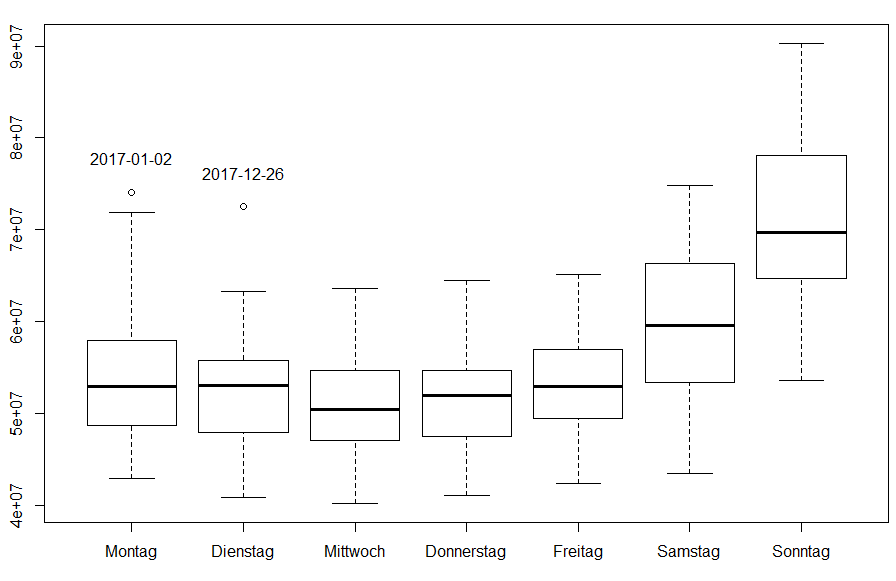
\includegraphics[width=0.9\linewidth]{../data/tv-week} 

}

\caption{\label{fig:fig1}The sum of TV viewing duration [seconds] by weekdays during 2017. On weekends more TV is watched than during the rest of the week. Festival days often behave like Sundays.}\label{fig:unnamed-chunk-2}
\end{figure}

\begin{figure}[H]

{\centering 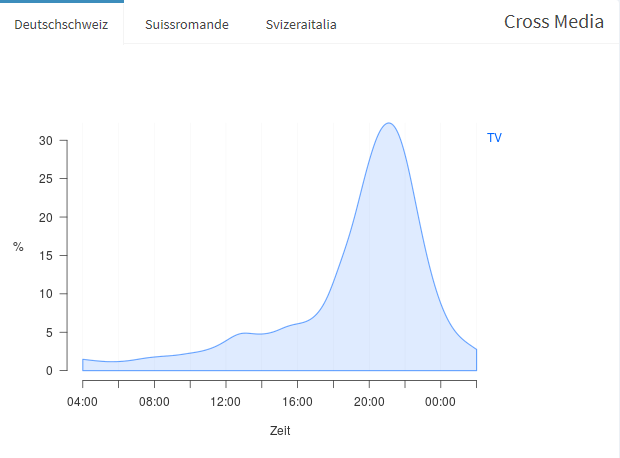
\includegraphics[width=0.9\linewidth]{../data/tv-day} 

}

\caption{\label{fig:fig2} The relative amount of TV viewing across time of the day. The curve is the average of all 365 days in 2017. In the market the peak around 20:00 o'clock is called Primetime. On weekends the curve is flatter.}\label{fig:unnamed-chunk-3}
\end{figure}


\end{document}
